\documentclass[12pt]{article}
\usepackage{graphicx}
\usepackage{caption}
\usepackage{geometry}
\usepackage[table]{xcolor}
\usepackage{titlesec}
\usepackage{fancyhdr}
\setlength{\headheight}{15pt}
\usepackage{array}
\usepackage{amsmath}
\geometry{margin=1in}
\usepackage{pgfplotstable}
\usepackage{tikz}
\usetikzlibrary{positioning,arrows.meta}
\pgfplotsset{compat=1.18}
\usepackage{hyperref}
\usepackage[font=small,labelfont=bf]{caption}


% Define custom colors
\definecolor{IonBlue}{RGB}{0,70,140}
\definecolor{IonGray}{RGB}{240,240,240}
\definecolor{IonAccent}{RGB}{200,50,50}

% Section formatting
\titleformat{\section}
  {\color{IonBlue}\normalfont\Large\bfseries}
  {\color{IonAccent}\thesection}{1em}{}

% Header and footer
\pagestyle{fancy}
\fancyhf{}
\fancyhead[L]{\color{IonBlue}HardHaQ '25 Ion Trap Challenge}
\fancyhead[R]{\color{IonAccent}\thepage}
\fancyfoot[C]{\color{IonBlue}Team Submission}

% Title
\title{\textcolor{IonBlue}{HardHaQ '25 Trapped Ion Problem Set Submission}}
\author{\textcolor{IonAccent}{Team Name:} \textit{Hard Nanos} \\ 
        \textcolor{IonAccent}{Members:} \textit{Nikhil, Rebanta, Lucas}}
\date{\ November 22 2025}

\begin{document}
\maketitle

\clearpage

\raggedright
\section{Introduction}
\subsection{Problem Overview}

The Ion Trap Challenge required us to modify an RF Paul trap to more effectively confine a single $\mathrm{Yb}^{+}$ ion using the combination of an oscillating and a static electric field inside of a vacuum environment. The primary components of the trap are the RF rods for radial confinement, DC endcaps for axial stability, and a vacuum region to minimize ion collisions with background gas molecules.
\begin{figure}[h!tbp]
    \centering
    \includegraphics[width=0.4\linewidth]{PDF_Visuals/Default_System.png}
    \captionof{figure}{Schematic of the ion trap components: RF rods, DC endcaps, and vacuum chamber. Each component plays a crucial role in achieving stable ion confinement.}
\end{figure}

Our team adopted a systematic strategy to tackle the ion trap challenge. We began by developing a clear understanding of the fundamental components of the RF Paul trap, recognizing that each element plays a distinct and indispensable role in achieving stable confinement. This foundational knowledge ensured that subsequent modifications were grounded in physical intuition rather than trial and error.



\subsection{RF Rods: Radial Confinement}

 The RF rods form the core of the quadrupole field. By applying an oscillating radiofrequency voltage, they generate a time-varying potential that counteracts the natural tendency of ions to escape. This produces dynamic stability in the radial plane through alternating focusing and defocusing forces.


\begin{figure}[h!tbp]
    \centering
    \includegraphics[width=0.4\linewidth]{PDF_Visuals/paul_trap_schematic.png}
    \captionof{figure}{Schematic of RF Paul trap showing RF rods, DC endcaps, and vacuum chamber. Radial confinement arises from oscillating RF rods which produce a time-varying quadrupole potential that traps the $\mathrm{Yb}^{+}$ ion dynamically in the radial plane.}  
\end{figure}
   
he electrodes in a quadrupole ion trap cannot simply be held at static voltages. A purely static quadrupole potential would violate \textbf{Earnshaw's theorem}, which states that no arrangement of static electric fields can create a stable equilibrium point for a charged particle in free space. The quadrupole potential is given by



\[
    \Phi(x,y,z) = \frac{V}{2r_0^2}(x^2 - y^2),
\]



where $V$ is the applied voltage and $r_0$ is the characteristic electrode spacing. This configuration confines ions along one radial axis while defocusing them along the orthogonal axis, producing a saddle-point potential that is inherently unstable.

To achieve confinement, the static voltages are replaced with an oscillating radio-frequency (RF) field. The rapid alternation between focusing and defocusing directions prevents the ion from escaping, and over many cycles the particle experiences an effective restoring force toward the trap center. This mechanism is analogous to the stabilization of the Kapitza pendulum, where fast oscillations create stability in an otherwise unstable system.

The time-averaged effect of the RF drive can be described by a \textbf{pseudo-potential}:



\[
    \Psi(r) = \frac{Q^2 V^2}{4 m \Omega^2 r_0^2} \, r^2,
\]



with $Q$ the ion charge, $m$ its mass, $\Omega$ the angular frequency of the RF drive, and $r$ the radial displacement. This effective potential is quadratic in $r$, resembling a harmonic oscillator well. Its strength scales with $V^2$ and decreases with increasing $m$ or $\Omega^{-2}$, meaning heavier ions are harder to confine while higher-frequency drives enhance stability.

In practice, trapped ions exhibit two types of motion: fast \textbf{micromotion} at the RF frequency and slower \textbf{secular motion} within the pseudo-potential well. The overall stability of trajectories is governed by the \textbf{Mathieu equations}, which define regions of confinement depending on the RF amplitude and frequency. This principle underlies devices such as the Paul trap and quadrupole mass filters, where precise tuning of the pseudo-potential enables selective confinement or ejection of ions based on their mass-to-charge ratio. 

\subsection{DC Endcaps: Axial Stability}

While the RF field provides dynamic stabilization in the radial plane, it cannot prevent ions from drifting freely along the longitudinal ($z$) axis of the ion trap. To address this limitation, \textbf{DC endcap electrodes} are introduced. These electrodes establish a static potential well along the trap axis, which provides axial confinement and completes the three-dimensional trapping scheme.

The axial potential can be expressed as



\[
    \Phi(z) = \frac{\kappa V_{\text{DC}}}{z_0^2} \, z^2,
\]



where $V_{\text{DC}}$ is the applied endcap voltage, $z_0$ is the characteristic axial dimension of the trap, and $\kappa$ is a geometry-dependent constant that accounts for electrode shape and spacing. This quadratic form resembles a harmonic oscillator potential, providing a restoring force that confines ions toward the trap center.

\begin{figure}[h!tbp]
\centering
    \includegraphics[width=0.4\linewidth]{PDF_Visuals/dc_endcaps.png}   
    \captionof{figure}{Illustration of DC endcaps providing axial confinement along the longitudinal axis of the trap.
    DC endcaps establish a static potential well along the trap axis, preventing axial drift and enabling long-term confinement when combined with the RF radial pseudopotential.}
\end{figure}

Physically, the DC endcaps play a complementary role to the RF field, as he RF drive ensures radial stability by generating a time-averaged pseudo-potential, while the DC endcaps supply a static potential that confines ions axially. Together, they create a three-dimensional trapping environment. 
In practice, the balance between RF and DC contributions must be carefully tuned. Too weak an endcap voltage leads to axial leakage, while excessive DC confinement can distort the radial pseudo-potential. 


\subsection{Vacuum Region: Isolation and Longevity}
\begin{figure}[h!tbp]
\centering

    \includegraphics[width=0.3\linewidth]{PDF_Visuals/vacuum_mean_free_path.png}
    \captionof{figure}{Diagram of mean free path in the vacuum region.
    Sparse background gas molecules increase the mean free path, reducing collisions and preserving ion coherence.}
\end{figure}

   Surrounding the electrodes is the vacuum region, which is not merely a passive enclosure but a critical component of the ion trap system. Its primary function is to drastically reduce the number of background gas molecules that could interact with the trapped ion. In the absence of sufficient vacuum, residual gas atoms can collide with the ion, causing unwanted momentum transfer, decoherence, and heating — all of which degrade trap performance and reduce confinement time. These collisions are especially problematic in precision applications such as quantum computing or spectroscopy, where long coherence times and minimal environmental noise are essential.

The effectiveness of the vacuum is quantified by the mean free path \(\lambda\), which represents the average distance an ion can travel before experiencing a collision. It is given by.


\[
\lambda = \frac{k_B T}{\sqrt{2} \pi d^2 P},
\]



where \(k_B\) is Boltzmann’s constant, \(T\) is the temperature, \(d\) is the effective diameter of the gas molecules, and \(P\) is the pressure. As pressure decreases, \(\lambda\) increases exponentially, meaning ions can traverse the trap volume without interference. Achieving ultra-high vacuum (UHV) conditions — typically below \(10^{-9}\) Torr — ensures that \(\lambda\) is orders of magnitude larger than the trap dimensions, effectively suppressing ion loss due to scattering.

From an engineering standpoint, maintaining UHV requires careful material selection, surface treatment, and bake-out procedures to eliminate outgassing. The trap chamber must be sealed with low-permeability materials and equipped with high-efficiency pumps such as turbomolecular or ion pumps. These measures collectively ensure that the vacuum region supports stable, long-duration trapping, enabling high-fidelity measurements and reliable ion manipulation.



\subsection{Interplay of Components}
\begin{figure}[h!tbp]
\centering
    \includegraphics[width=0.5\linewidth]{PDF_Visuals/trap_interplay.png}
    \captionof{figure}{Composite schematic showing RF rods, DC endcaps, and vacuum chamber working together.
    Stable confinement emerges only when dynamic radial forces, static axial potentials, and isolation are combined.}
    \end{figure}

    Together, these three components—RF rods for radial confinement, DC endcaps for axial stability, and the vacuum region for isolation, form a carefully balanced system. Each element addresses a limitation of the others: the RF rods alone cannot trap ions, the DC endcaps alone cannot prevent radial escape, and neither can function effectively without the vacuum. 

    Stable confinement emerges only when dynamic and static potentials are combined in a low-pressure environment, reflecting the fundamental design principle of the Paul trap. The oscillating RF field generates a pseudo-potential that stabilizes radial motion, while the DC endcaps create a static quadratic potential well along the longitudinal axis. The vacuum ensures that these forces act coherently over longer timescales.

    Mathematically, the total potential experienced by an ion in the trap can be expressed as the superposition of RF and DC contributions:
    

\[
    \Phi(x,y,z,t) = \Phi_{\text{RF}}(x,y,t) + \Phi_{\text{DC}}(z),
    \]


    where
    

\[
    \Phi_{\text{RF}}(x,y,t) = \frac{V_{\text{RF}}}{2r_0^2}(x^2 - y^2)\cos(\Omega t),
    \quad
    \Phi_{\text{DC}}(z) = \frac{\kappa V_{\text{DC}}}{z_0^2}z^2.
    \]



    This interplay is not just additive but synergistic: the RF and DC fields together establish a three-dimensional potential slope in which ions can be localized with high precision. The vacuum region amplifies this stability by extending ion lifetimes.



\section{Mathematical Framework}
\subsection{Shorthand useful relations}
The Mathieu parameter (radial) is
\begin{equation}
  q \;=\; \frac{2 Q V}{m r_0^2 \Omega^2}.
\end{equation}
% Definitions introduced at first use
Here $Q$ is the ion charge (C), $m$ is the ion mass (kg), $V$ is the RF peak amplitude (V), $\Omega$ is the RF angular frequency (rad\,s$^{-1}$), and $r_0$ is the characteristic trap radius (m).
The secular frequency (radial secular motion) in the small-$q$ limit is approximated by
\begin{equation}
  \omega_{\mathrm{sec}} \;\approx\; \frac{q}{2\sqrt{2}}\,\Omega
  \;=\; \frac{Q V}{\sqrt{2}\, m r_0^2 \Omega}.
\end{equation}

\subsection[Pseudopotential depth (U_depth)]{Pseudopotential depth (\(U_{\mathrm{depth}}\))}
\subsubsection{Governing formula}
The time-averaged pseudopotential (in 1D radial coordinate $r$ for an ideal quadrupole) is
\[
\Psi(r) \;=\; \frac{Q^2}{4 m \Omega^2}\,|\mathbf{E}_{\rm rf}(r)|^2.
\]
% Definition: pseudopotential
\par
\noindent Here $\Psi(\mathbf r)$ is the time-averaged pseudopotential (J).
For the ideal quadrupole field amplitude $|\mathbf{E}_{\rm rf}|\!\sim\! V r / r_0^2$, this gives a quadratic pseudopotential:
\[
\Psi(r) \;=\; \kappa\,\frac{Q^2 V^2}{4 m \Omega^2 r_0^4}\; r^2,
\]
so a characteristic \emph{trap depth} (energy scale between center and effective boundary $r\!\sim\!r_0$) is commonly approximated as
\begin{equation}\label{eq:Udepth}
  U_{\rm depth} \;\approx\; \kappa\,\frac{Q^2 V^2}{4 m \Omega^2 r_0^2}.
\end{equation}
\par
\noindent Here $U_{\rm depth}$ denotes the trap depth (J) and $\kappa$ is a dimensionless geometry factor (order unity).
An alternative useful form in terms of the Mathieu parameter $q$ is
\begin{equation}\label{eq:Udepth_q}
  U_{\rm depth} \;=\; \kappa\,\frac{m \Omega^2 r_0^2}{16}\; q^2.
\end{equation}

\subsubsection{How each variable affects depth}
\begin{itemize}
  \item \textbf{RF amplitude $V$:} $U_{\rm depth}\propto V^2$. \emph{Increasing $V$ increases depth quadratically.}
  \item \textbf{Drive frequency $\Omega$:} $U_{\rm depth}\propto 1/\Omega^2$. \emph{Increasing $\Omega$ reduces depth (inverse square).}
  \item \textbf{Trap size $r_0$:} $U_{\rm depth}\propto 1/r_0^2$. \emph{Increasing $r_0$ decreases depth (inverse square).}
  \item \textbf{Ion properties $Q,m$:} $U_{\rm depth}\propto Q^2/m$. Higher charge increases depth; heavier mass decreases depth.
  \item \textbf{Geometry $\kappa$:} improves depth linearly with $\kappa$ (ideal electrodes have $\kappa\!\approx\!1$).
\end{itemize}

\subsubsection{Practical remarks and trade-offs}
\begin{itemize}
  \item Increasing $V$ increases $q$. Large $q$ invalidates the pseudopotential approximation and increases micromotion.
\end{itemize}

\subsection{Center offset ({$x_0$}) — static displacement and micromotion}
\subsubsection{Governing formula}
If a stray DC electric field $E_{\rm dc}$ exists at the trap center, it exerts a force $Q E_{\rm dc}$ on the ion. Balance this against the secular restoring force $m \omega_{\mathrm{sec}}^2 x$ to obtain the static displacement (offset) $x_0$:
\begin{equation}\label{eq:x0}
  x_0 \;=\; \frac{Q E_{\rm dc}}{m \omega_{\mathrm{sec}}^2}.
\end{equation}
\par
\noindent where $E_{\mathrm{dc}}$ is the stray DC electric field (V/m) producing the static offset.
Using the small-$q$ expression for $\omega_{\mathrm{sec}}$,
\[
\omega_{\mathrm{sec}} \approx \frac{Q V}{\sqrt{2}\, m r_0^2 \Omega},
\]
we can express $x_0$ in terms of trap parameters:
\begin{equation}\label{eq:x0_expanded}
  x_0 \;\approx\; \frac{Q E_{\rm dc}}{m}\left(\frac{\sqrt{2}\, m r_0^2 \Omega}{Q V}\right)^{\!2}
  \;=\; \frac{2 m r_0^4 \Omega^2}{Q V^2}\;E_{\rm dc}.
\end{equation}

\subsubsection{Excess micromotion amplitude (leading order)}
For small $q$ the amplitude of \emph{excess} micromotion driven at RF frequency is approximately proportional to $q$ times the static offset:
\begin{equation}
  x_{\rm mm} \;\approx\; \frac{q}{2}\,x_0.
\end{equation}
Kinetic energy associated with excess micromotion scales as $\sim \tfrac{1}{2} m (\Omega x_{\rm mm})^2$.

\subsubsection{How each variable affects center offset}
\begin{itemize}
  \item \textbf{Stray field $E_{\rm dc}$:} $x_0\propto E_{\rm dc}$ (linear). More stray field $\Rightarrow$ larger offset.
  \item \textbf{Secular stiffness $\omega_{\rm sec}$:} $x_0\propto 1/\omega_{\rm sec}^2$. Stronger confinement (higher $\omega_{\rm sec}$) $\Rightarrow$ smaller $x_0$.
  \item \textbf{RF amplitude $V$:} Increasing $V$ increases $\omega_{\rm sec}$ (for fixed $\Omega$ and $r_0$) and thus reduces $x_0$; but increasing $V$ also increases $q$ and so multiplies offset into micromotion amplitude.
  \item \textbf{Drive frequency $\Omega$:} Appears in $\omega_{\mathrm{sec}}$ inversely; higher $\Omega$ (for fixed $V$) tends to reduce $x_0$ via $\omega_{\mathrm{sec}}$ formula in practice.
  \item \textbf{Trap size $r_0$:} Larger $r_0$ reduces secular frequency (for fixed $V,\Omega$) so $x_0$ grows with $r_0$.
\end{itemize}

\subsubsection{Minimization strategies}
\begin{itemize}
  \item \textbf{Increase secular stiffness:} Raise $V$ or reduce $r_0$ (within other constraints) to reduce $x_0$.
  \item \textbf{Balance trade-offs:} Increasing $V$ reduces $x_0$ but increases $q$ (and thus micromotion amplitude $x_{\rm mm}\propto q x_0$). Optimize to minimize residual micromotion energy.
\end{itemize}

\subsection{RF power and power-per-depth (\texorpdfstring{$P/U_{\mathrm{depth}}$}{P/U_depth})}
\subsubsection{Model for RF power}
The RF power is modelled by the following equation extracted from the COMSOL file:
\begin{equation}\label{eq:Pdiss}
  P_{\mathrm{est}} \;=\; 10^{3}\left(\omega_{\mathrm{sec}}\big(\varepsilon\pi L\big)\frac{V_{\mathrm{rf}}}{\sqrt{2}}\right)^{2}
\end{equation}
Here $V_{\mathrm{rf}}$ is the RF peak amplitude. In practice, $P_{\mathrm{est}}$ also depends on the effective electrode capacitance and series resistance of the RF drive and electrode structure (but, we assume it is negligible).

\subsubsection{Power per depth}
Combine \eqref{eq:Pdiss} with the depth formula \eqref{eq:Udepth} which scales as $U_{\rm depth}\propto V^2$. Eliminating $V^2$ yields:
\begin{equation}\label{eq:PoverU_raw}
  \frac{P_{\mathrm{est}}}{U_{\rm depth}}
  \;\propto\; \frac{10^{3}\left(\omega_{\mathrm{sec}}\big(\varepsilon\pi L\big)\frac{V_{\mathrm{rf}}}{\sqrt{2}}\right)^{2}}{\;\kappa\,\frac{m \Omega^2 r_0^2}{16}\; q^2\;}  \Rightarrow ...
  \Rightarrow \frac{P_{\mathrm{est}}}{U_{\rm depth}} \propto \frac{10^{3}(\varepsilon\pi L)^{2}  V_{\mathrm{rf}}^{2}}{\kappa m r_{0}^{2}}.
\end{equation}
where the constant prefactor depends on the precise definitions used for $U_{\rm depth}$ and $P_{\rm est}$; the displayed scaling is the relevant design dependence.

\subsubsection{How each variable affects $P/U_{\rm depth}$}
\begin{itemize}
  \item \textbf{Trap size $r_0$:} $P/U_{\rm depth}\propto r_0^2$ (scales with trap area/size) — larger traps cost more power per depth.
  \item \textbf{Ion properties:} $P/U_{\rm depth}\propto m/Q^2$ — heavier ions increase power per depth; higher ionic charge reduces it.
  \item \textbf{RF voltage $V_{\rm rf}$:} $P/U_{\mathrm{depth}}\propto V_{\rm rf}^{2}$;  
      smaller $V_{\rm rf}$ reduces power cost.
  \item \textbf{Electrode length $L$:} $P/U_{\mathrm{depth}}\propto L^{2}$;  
      smaller $L$ reduces power cost if the quadrupole field quality is preserved.

\end{itemize}

\subsubsection{Minimization of $P/U_{\rm depth}$}
\begin{enumerate}
  \item \textbf{Choose moderate $\Omega$:} Avoid excessively high drive frequencies unless required for stability/performance.
  \item \textbf{Reduce $r_0$ where acceptable:} Smaller traps require less RF voltage for a given depth.
\end{enumerate}

\section{Optimization}

\subsection{Potential Approaches}

There are two main strategies for optimizing the ion trap design: (1) modifying the geometries of the trap electrodes, and (2) adjusting the operating parameters such as voltages, frequencies, and characteristic dimensions of the RF Paul trap. Each approach offers distinct advantages and limitations.

\paragraph{Optimizing Operating Parameters}
Tuning parameters such as RF voltage amplitude, drive frequency, and endcap potentials is often the most accessible method of optimization.
\begin{itemize}
    \item \textbf{Pros:}
    \begin{itemize}
        \item Rapid and flexible adjustments without requiring physical redesign of the trap.
        \item Enables fine control over stability regions defined by the Mathieu equations.
        \item Lower cost and shorter iteration cycles, since changes are implemented electronically.
        \item Useful for adapting a single trap geometry to different ion species or experimental conditions.
    \end{itemize}
    \item \textbf{Cons:}
    \begin{itemize}
        \item Limited by the intrinsic geometry of the electrodes; cannot overcome fundamental design constraints.
        \item High voltages or frequencies may introduce technical challenges such as dielectric breakdown, heating, or increased micromotion.
        \item Optimization may be bounded by available electronics and power-handling capabilities.
    \end{itemize}
\end{itemize}

\paragraph{Modifying Trap Geometries}
Altering electrode shapes, spacings, or overall trap dimensions provides a more fundamental route to optimization.
\begin{itemize}
    \item \textbf{Pros:}
    \begin{itemize}
        \item Directly improves field uniformity and reduces anharmonicities in the pseudo-potential.
        \item Can expand stability regions and reduce sensitivity to parameter fluctuations.
        \item Enables custom designs tailored to specific applications (e.g., quantum computing, precision spectroscopy).
    \end{itemize}
    \item \textbf{Cons:}
    \begin{itemize}
        \item Requires fabrication of new hardware, which is costly and time-consuming.
        \item Less flexible once built; geometry changes cannot be easily undone.
        \item Complex geometries may introduce alignment issues or machining tolerances that degrade performance.
    \end{itemize}
\end{itemize}

\begin{figure}[h!tbp]
    \centering
    \includegraphics[width=0.8\linewidth]{PDF_Visuals/Default_Parameters.png}
    \captionof{figure}{Default operating parameters of the RF Paul trap.
    Initial voltages, frequencies, and dimensions set the baseline before any optimization.}
\end{figure}

Given the benefits of both optimizing values and geometries, our team elected to focus primarily on parameter optimization at the beginning of the challenge. This approach allowed us to rapidly iterate and explore a wide parameter space without the overhead of physical redesign. By leveraging computational tools to simulate trap performance under varying conditions, we could identify optimal settings that maximized trap depth, minimized offset, and controlled power consumption.
Over the course of the challenge, we also explored geometric modifications to further enhance performance based on insights gained from our algorithmic parameter sweeps.

\subsection{Optimizing Parameters}


In our approach to optimizing the values of the parameters, we developed a Python script that interfaces with COMSOL's \texttt{mph} module to iteratively adjust key operating parameters of the ion trap model. The goal was to maximize trap depth while minimizing offset and power consumption, all within physically meaningful bounds.
Because of the nature of the offset, minimizing it proved to be rather difficult, so the ratio of depth to power consumption was the main objective of the optimization script.

\vspace{\baselineskip}

The script attempts to optimize physical parameters of an ion trap model in COMSOL by coupling
the \texttt{mph} Python interface with SciPy's \texttt{minimize} routine. The workflow can be
summarized as follows:

\begin{itemize}
    \item \textbf{Baseline, Targets, and Weights:} 
    Baseline values are taken from the COMSOL GUI and serve as the starting point. 
    Target values specify desired outcomes (e.g., trap depth $\geq 5$ eV, offset $\approx 0$ mm, 
    power $\approx 10$ mW). Each objective is assigned a weight to reflect its relative importance, and each objective is designed to be just beyond what we thought was realistically achievable.

    \item \textbf{Bounds:} 
    Each parameter is constrained to physically meaningful ranges 
    (e.g., $0 \leq V_{\mathrm{rf}} \leq 1000$, $10^{6} \leq f \leq 10^{8}$). 
    These bounds are used to normalize parameters into the unit cube $[0,1]^n$ for optimization 
    and then denormalize them back to physical units before evaluation.

    \item \textbf{Objective Function:} 
    The function computes normalized scores relative to targets:
    

\[
        \text{depth score} = \frac{\text{depth}}{\text{target depth}}, \quad
        \text{offset score} = \frac{\text{target offset}}{\text{actual offset}}, \quad
        \text{power score} = \frac{\text{target power}}{\text{actual power}}.
    \]


    These are combined into a weighted sum. Higher scores indicate better performance.

    \item \textbf{Trial Execution:} 
    For each candidate parameter set, values are pushed into the COMSOL model, 
    the study is solved, and metrics such as trap depth, offset, and power are extracted. 
    Penalties are applied if results are unphysical. The optimizer minimizes the negative score, 
    effectively maximizing performance.

    \item \textbf{Optimization Loop:} 
    The Nelder--Mead algorithm iteratively proposes new parameter sets in normalized space, 
    evaluates them via COMSOL, and updates its simplex until convergence or iteration limits are reached.

    \item \textbf{Logging:} 
    Each trial's parameters and results are written to a CSV file for record-keeping and more in-depth analysis.
\end{itemize}
\begin{figure}[h!tbp]
\centering
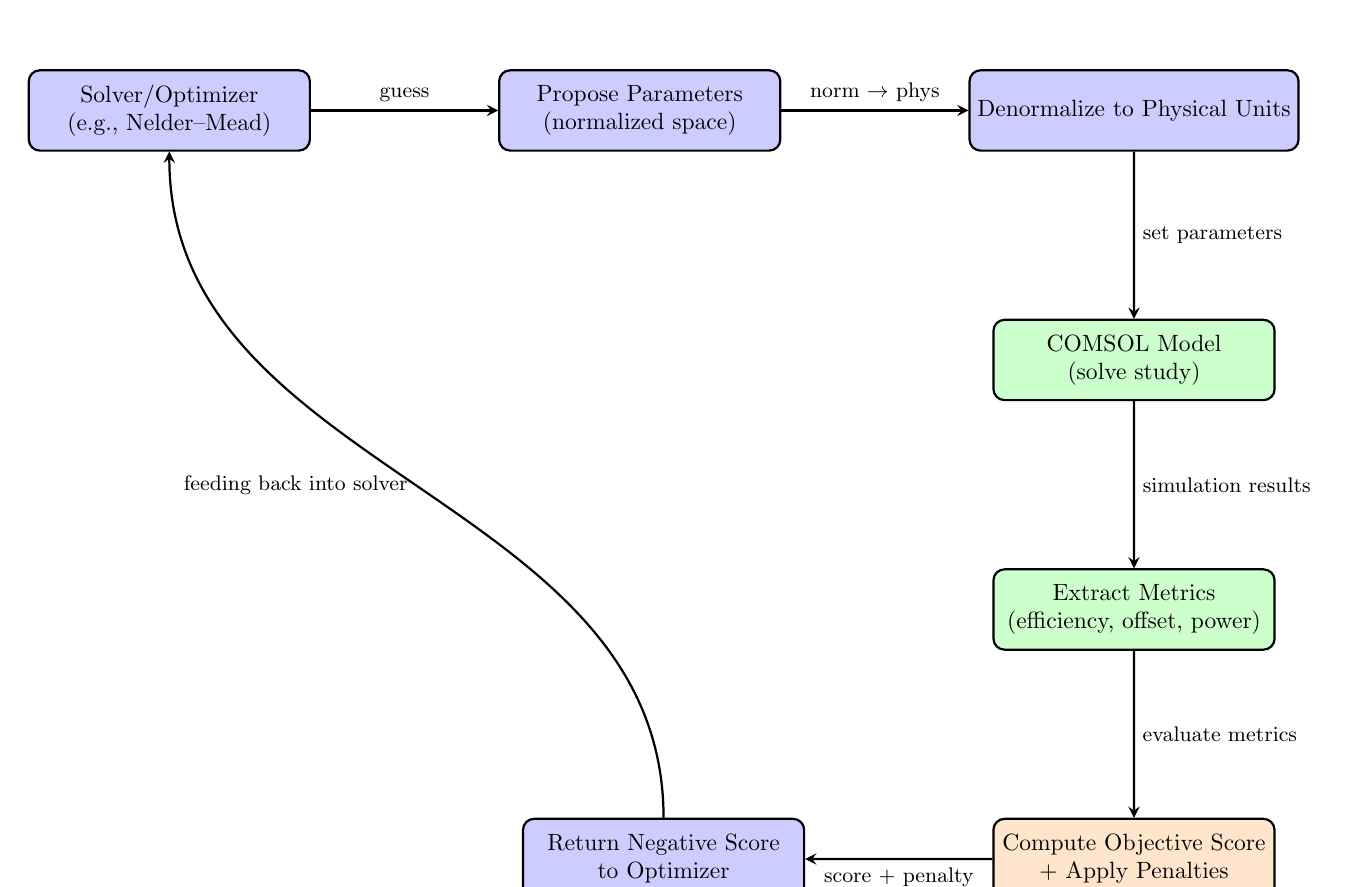
\begin{tikzpicture}[scale=0.85, transform shape, node distance=2.5cm and 2.8cm, >=stealth, thick]
    % Styles
    \tikzstyle{optimizer}=[rectangle, draw, rounded corners, fill=blue!20, align=center, minimum width=4.2cm, minimum height=1.2cm]
    \tikzstyle{comsol}=[rectangle, draw, rounded corners, fill=green!20, align=center, minimum width=4.2cm, minimum height=1.2cm]
    \tikzstyle{objective}=[rectangle, draw, rounded corners, fill=orange!20, align=center, minimum width=4.2cm, minimum height=1.2cm]

    % Horizontal top row
    \node (start) [optimizer] {Solver/Optimizer \\ (e.g., Nelder--Mead)};
    \node (params) [optimizer, right=of start] {Propose Parameters \\ (normalized space)};
    \node (denorm) [optimizer, right=of params] {Denormalize to Physical Units};

    % Vertical drop
    \node (comsol) [comsol, below=of denorm] {COMSOL Model \\ (solve study)};
    \node (metrics) [comsol, below=of comsol] {Extract Metrics \\ (efficiency, offset, power)};
    \node (objective) [objective, below=of metrics] {Compute Objective Score \\ + Apply Penalties};

    % Horizontal return path
    \node (update) [optimizer, left=of objective] {Return Negative Score \\ to Optimizer};

    % Arrows with labels and routing
    \draw[->] (start.east) -- (params.west) node[midway,above] {\small guess};
    \draw[->] (params.east) -- (denorm.west) node[midway,above] {\small norm $\to$ phys};
    \draw[->] (denorm.south) -- (comsol.north) node[midway,right] {\small set parameters};
    \draw[->] (comsol.south) -- (metrics.north) node[midway,right] {\small simulation results};
    \draw[->] (metrics.south) -- (objective.north) node[midway,right] {\small evaluate metrics};
    \draw[->] (objective.west) -- (update.east) node[midway,below] {\small score + penalty};
    \draw[->] (update.north) to[out=90,in=270] node[midway,left] {\small feeding back into solver} (start.south);

\end{tikzpicture}
\caption{simulation-driven optimization loop using SciPy and COMSOL. Parameters are proposed, evaluated, and scored before looping back.}
\label{fig:iontrap-optimization-loop-horizontal}
\end{figure}



In summary, the script establishes a simulation-driven optimization loop:

\clearpage
\subsection{Geometric Modification}

In addition to parameter optimization, we explored modifications to the electrode geometry itself. 
The change we ultimately attempted to implement was a reshaping of the electrodes into an 
hourglass profile. By tapering the electrode structure, the constriction is supposed to generate additional 
vertical confinement forces that pushes the ion inward along the $z$-axis. The intended effect of this is to provide direct 
assistance to the endcap electrodes in minimizing axial motion.

The hourglass geometry also was intended to assist in reducing offset. Its symmetric focusing of the 
pseudo-potential toward the trap center conceptually would help stabilize the ion's position while maintaining 
radial uniformity.

Unfortunately, we were unable to fully implement and test this geometric modification
within the COMSOL environment. However, we believe that such geometric changes hold promise for further enhancing
trap performance beyond what parameter tuning alone can achieve.

\begin{figure}[h!tbp]
    \centering
    \includegraphics[width=0.8\linewidth]{PDF_Visuals/hourglass.jpg}
    \captionof{figure}{Pictured above is a conceptual rendering of the hourglass electrode geometry.
    The tapered design aims to enhance axial confinement and reduce offset by focusing the pseudo-potential toward the trap center.}
\end{figure}


\clearpage
\section{Conclusion}
Through parameter optimization, our team achieved a final Trap Metrics table with the following key results:
\begin{table}[h!]
\centering
\caption{Optimization Results for Ion Trap Parameters}
\resizebox{\textwidth}{!}{%
\begin{tabular}{|c|c|c|c|c|c|c|c|c|c|c|c|c|c|}
\hline
\textbf{V\_rf} & \textbf{V\_dc} & \textbf{V\_endcap} & \textbf{rod\_spacing} & \textbf{rod\_radius} & \textbf{rod\_length} & \textbf{endcap\_offset} & \textbf{endcap\_rad} & \textbf{endcap\_thick} & \textbf{f} \\
\hline
0.3887 & 76.5038 & 8.3279 & 0.00586 & 0.00179 & 0.04221 & 0.00096 & 0.00608 & 0.00052 & 9514109.64 \\
\hline
\end{tabular}%
}
\end{table}

\begin{table}[h!]
\centering
\caption{Trap Metrics from COMSOL Global Evaluation}
\begin{tabular}{|c|c|c|c|c|c|c|c|}
\hline
\textbf{depth\_eV} & \textbf{minU\_eV} & \textbf{maxU\_eV} & \textbf{trap\_x} & \textbf{trap\_y} & \textbf{trap\_z} & \textbf{offset\_mm} & \textbf{P\_est\_mW} \\
\hline
0.9755 & 74.3162 & 75.2917 & 0 & -5.0E-6 & 0.01 & 10.0000 & 0.01083 \\
\hline
\end{tabular}
\end{table}

These results reflect an incredible improvement over the baseline configuration, demonstrating the effectiveness of our optimization strategy in enhancing trap performance without geometrically changing the electrode structure.



\begin{itemize}
    \item Exported Trap Metrics table (.txt file)
    \item Screenshot(s) of geometry and potential distribution
    \item Modified COMSOL file (.mph)
    \item Written summary (this document)
\end{itemize}

\end{document}